\documentclass{article}
\usepackage{graphicx}
\usepackage{float}

\usepackage{booktabs}
\usepackage{tabularx}
\usepackage{hyperref}
\usepackage{pdflscape}
\usepackage{ltablex}
\usepackage{lipsum}

\keepXColumns

% Defines new column types that use ragged right so the table doesn't look awful
\newcolumntype{Y}{>{\raggedright\arraybackslash}X}
\newcolumntype{P}[1]{>{\raggedright\arraybackslash}p{#1}}

\hypersetup{
    colorlinks=true,       % false: boxed links; true: colored links
    linkcolor=red,          % color of internal links (change box color with linkbordercolor)
    citecolor=green,        % color of links to bibliography
    filecolor=magenta,      % color of file links
    urlcolor=cyan           % color of external links
}

\title{Hazard Analysis\\\progname}

\author{\authname}

\date{}

%% Comments

\usepackage{color}

\newif\ifcomments\commentstrue %displays comments
%\newif\ifcomments\commentsfalse %so that comments do not display

\ifcomments
\newcommand{\authornote}[3]{\textcolor{#1}{[#3 ---#2]}}
\newcommand{\todo}[1]{\textcolor{red}{[TODO: #1]}}
\else
\newcommand{\authornote}[3]{}
\newcommand{\todo}[1]{}
\fi

\newcommand{\wss}[1]{\authornote{magenta}{SS}{#1}} 
\newcommand{\plt}[1]{\authornote{cyan}{TPLT}{#1}} %For explanation of the template
\newcommand{\an}[1]{\authornote{cyan}{Author}{#1}}

%% Common Parts

\newcommand{\progname}{Software Engineering} % PUT YOUR PROGRAM NAME HERE
\newcommand{\authname}{Team 8, RLCatan
\\ Rebecca Di Filippo
\\ Jake Read
\\ Matthew Cheung
\\ Sunny Yao} % AUTHOR NAMES

\usepackage{hyperref}
    \hypersetup{colorlinks=true, linkcolor=blue, citecolor=blue, filecolor=blue,
                urlcolor=blue, unicode=false}
    \urlstyle{same}
                                


\begin{document}

\maketitle
\thispagestyle{empty}

~\newpage

\pagenumbering{roman}

\begin{table}[hp]
\caption{Revision History} \label{TblRevisionHistory}
\begin{tabularx}{\textwidth}{llX}
\toprule
\textbf{Date} & \textbf{Developer(s)} & \textbf{Change}\\
\midrule
2025-10-05 & Jake Read, Sunny Yao, Created first version of document.\\

\bottomrule
\end{tabularx}
\end{table}

~\newpage

\tableofcontents
\listoftables
\listoffigures

~\newpage

\pagenumbering{arabic}


\section{Introduction}\label{sec:introduction}


\subsection{Background}\label{subsec:background}
Our project, RLCatan, is an AI-assisted tool that observes a physical game of Catan via camera feed and provides real-time strategic advice to players.
The system integrates computer vision, game state modeling, and AI-based decision-making.

\subsection{Hazard Definition}\label{subsec:hazard-definition}
A hazard is defined as a property or condition in the system together
with a condition in the environment that has the potential to cause harm or
damage. We define harm as the underperformance of our system
that leads to the incorrect instruction of players. In addition, we consider
disruption of play, loss of game data/state as harm.


\section{Scope and Purpose of Hazard Analysis}\label{sec:scope-and-purpose-of-hazard-analysis}



The loss that can be incurred because of the hazards include the
forfeiture or inability to continue a game of Catan. This can affect the
user experience of our software and lead to a loss of trust in the product.


\section{System Boundaries and Components}\label{sec:system-boundaries-and-components}



Components: 
\begin{itemize}

\item User Interface
\item Game State Manager
\item AI Model
\item Computer Vision Model
\item Reinforcement Learning Environment
\item Image Queue
\item Game State Database

\end{itemize}

\begin{figure}[H]
    \centering
    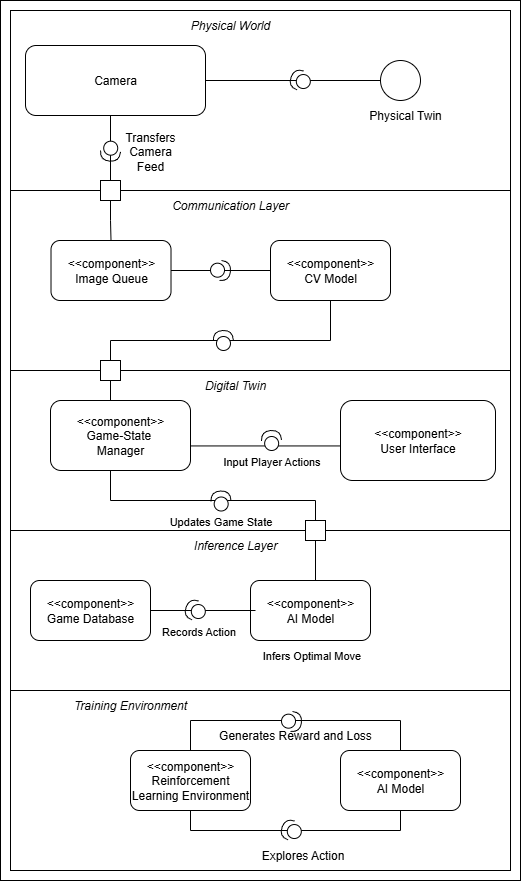
\includegraphics[width=\textwidth]{Component_Diagram_final.png}
    \caption{\textit{System components: User Interface, Game State Digital Twin, AI Model, Board Representation, Game State Database}}
    \label{fig:component-diagram}
\end{figure}

\section{Critical Assumptions}\label{sec:critical-assumptions}



We assume that the users of our system will be familiar with the rules of Catan and
know how to play the game. Another assumption is that the users will have a basic understanding
of how to interact with a digital interface. Finally, we assume that existing consumer
hardware will be able to run full-depth processing of our AI model.

\section{Failure Mode and Effect Analysis}\label{sec:failure-mode-and-effect-analysis}


% Finally, a table that spans multiple pages and doesn't look horrendous, only took 2 hours to get the formatting right...
\begin{landscape}
    The following FMEA table summarizes identified hazards, their effects and causes, and corresponding mitigation strategies.
    Each row represents a unique failure mode for one of the components listed in Figure~\ref{fig:component-diagram}.

    % Layout setup
    \renewcommand{\arraystretch}{1.3}
    \begin{tabularx}{\linewidth}{|P{2.5cm}|Y|Y|Y|Y|P{1cm}|P{1cm}|}

        % Header
        \caption{Failure Mode and Effect Analysis (FMEA)} \label{TblFMEA} \\
        \hline
        \textbf{Component} &
        \textbf{Failure Modes} &
        \textbf{Effects of Failure} &
        \textbf{Causes of Failure} &
        \textbf{Recommended Action} &
        \textbf{SR} &
        \textbf{Ref.} \\
        \hline
        \endfirsthead

        % Subsequent pages header
        \hline
        \textbf{Component} &
        \textbf{Failure Modes} &
        \textbf{Effects of Failure} &
        \textbf{Causes of Failure} &
        \textbf{Recommended Action} &
        \textbf{SR} &
        \textbf{Ref.} \\
        \hline
        \endhead

        % Prompt that the table continues
        \hline
        \multicolumn{7}{r}{\textit{Continued on next page}} \\
        \endfoot

        % No footer on last page
        \hline
        \endlastfoot

        % Table Rows...
        Board Representation &
        Incorrect parsing of the physical board state (e.g., misidentifies road or settlement). &
        AI advice is based on false information, leading to invalid or poor recommendations. &
        - CV model misclassifies pieces due to lighting, angle, or occlusion. &
        Give the option for users to manually confirm the parsed board state before generating advice. &
        SR-1 &
        H1-a \\

        \hline

        Game State Digital Twin &
        Loss of synchronization between physical game and digital twin. &
        System provides advice for the wrong game state, disrupting play. &
        - Failure to read new game state to model. \newline - Additional moves made by players after CV scan. &
        Provide a resynchronization mechanism, such as an option to rescan the board or manually enter current state. &
        SR-2 &
        H2-a \\

        \hline

        AI Model &
        AI suggests an illegal or nonsensical move. &
        Users may become confused or game flow disrupted if they attempt an invalid action. &
        -AI loses track of game state. \newline AI misinterprets rules. \newline - Rules are not properly encoded. &
        AI-suggested moves are validated against the official rules of Catan before display. &
        SR-3 &
        H3-a \\

        &
        Trained model diverges from expected behaviour. &
        System makes suboptimal or inconsistent suggestions. &
        - Model overfits. \newline - Inconsistencies in training environment. \newline - Poor heuristics. &
        Maintain rollback capability, and allow user to select older models. &
        SR-12 &
        H3-b \\


        \hline

        User Interface &
        Advice not displayed on time. &
        Player's turn timer runs out, causing them to miss their turn as they wait. &
        - Model takes too long to compute next move. \newline - There are delays in CV processing. &
        Limit the processing time of the model or timeout early and inform user of failure before their turn ends. &
        SR-4 \newline SR-5 &
        H4-a \\

        &
        Incorrect or confusing rendering of the game state. &
        Players misinterpret advice or system status, leading to wrong actions. &
        Suggested move is not easy to quickly spot on the displayed board. &
        Visually distinguish the move(s) suggested by AI, e.g., using highlights or arrows. &
        SR-9 &
        H4-b \\

        \hline

        Game State Database &
        Failure to save game states. &
        LLM is unable to summarize "what could have been" from previous game states. &
        - Game moves too quickly for state to be saved (Mostly applicable to bot vs. bot games). &
        Ensure that the current game state is saved correctly before the recommended move is sent to the user. &
        SR-6 &
        H5-a \\

        \hline

        Communication Layer (Phone/Server) &
        Dropped connection between user device and processing server. &
        Advice delayed or not delivered, leading to disrupted play. &
        - External server goes down \newline - WiFi connectivity issues occur. &
        Attempt to reconnect, and notify the user that connection has dropped. &
        SR-7 \newline SR-8 &
        H6-a \\

        \hline

        Camera Feed &
        Game stream is cut off. &
        The model will have no data with which to make predictions, so no move will be displayed to the user. &
        - Recording device runs out of battery. \newline - Recording device is damaged. &
        Notify user when stream cuts out, to give them a chance to fix it, or at least be aware of why move predictions have ended. &
        SR-10 &
        H7-a \\

        &
        Camera is unable to view entire board. &
        Model receives incomplete or garbage data. &
        - Camera is misaligned. \newline - Camera is blocked by some object (e.g. another player). &
        Detect a lack of data from the stream and warn user that camera may be misaligned or blocked. &
        SR-11 &
        H7-b \\

        &
        Game streams/snapshots contain identifiable players/background content.
        &
        Unintended sharing or exposure of personal information. &
        - Limit recording to within the bounds of the board. &
        SR-13 &
        H7-c \\

    \end{tabularx}
\end{landscape}

\section{Safety and Security Requirements}\label{sec:safety-and-security-requirements}


The following safety and security requirements have been derived from the hazard analysis above.
Each requirement is traced to a hazard in the FMEA table (Table~\ref{TblFMEA}):

\begin{itemize}
    \item SR-1: The system shall enable users to manually confirm the parsed board state before generating advice.
    \item SR-2: The system shall provide a resynchronization mechanism (manual correction or re-scan).
    \item SR-3: The system shall validate all AI-suggested moves against the official rules of Catan before display.
    \item SR-4: The system shall ensure advice is displayed within 5 seconds of request.
    \item SR-5: The system shall provide a clear error message if advice cannot be generated.
    \item SR-6: The system shall ensure current game state is saved correctly before recommending move(s) to the user.
    \item SR-7: The system shall notify the user of connection loss within 5 seconds.
    \item SR-8: The system shall attempt automatic reconnection at least 3 times before failing.
    \item SR-9: The system shall visually distinguish the move(s) suggested by AI.
    \item SR-10: The system shall notify the user in the event board streaming ceases.
    \item SR-11: The system shall warn the user when incomplete game data is read where possible.
    \item SR-12: The system shall enable the user to roll-back to previous model versions.
    \item SR-13: The system shall only capture and process game board area, not player faces or personal content.
\end{itemize}


\section{Roadmap}\label{sec:roadmap}

\subsection{Requirements Planned During Capstone}\label{subsec:requirements-planned-during-capstone}
The following requirements will be implemented as part of the capstone timeline:
\begin{itemize}
    \item SR-1: Being able to confirm the board state is crucial in the early stages to ensure the system is functioning correctly.
          It will be valuable for both users and developers to have this feature implemented early.
    \item SR-2: Resynchronization is important to maintain the integrity of the game state.
          This feature will help recover from potential errors in board state detection, which is likely to occur during initial testing and development.
    \item SR-3: If the AI suggests illegal moves, the entire purpose of the system is defeated.
          This requirement is essential to ensure the system provides valid advice.
    \item SR-5: Clear error messages are important not only for user experience but also for debugging during development, so it makes sense to add them early.
    \item SR-6: The issues caused by game states not being saved correctly will likely be a problem primarily in bot vs. bot games.
          This will be most useful while training the AI, which is naturally within the scope of the capstone.
    \item SR-9: Clear visualization of AI suggestions is important for user experience and should be relatively straightforward to implement.
          This will help users quickly understand the AI's advice, which is a core functionality of the system.
    \item SR-12: We will likely make mistakes when training the model, so the ability to roll back to old model versions will be critical in development.
\end{itemize}

\subsection{Delayed Requirements}\label{subsec:delayed-requirements}
The following requirements are planned for future implementation:
\begin{itemize}
    \item SR-4: While timely advice is important, it may be challenging to guarantee a strict time limit during the initial development phase.
    \item SR-7: Connection loss handling is important, but it may be less critical during initial development when the focus is on core functionalities.
          For now, we'll assume a stable connection.
    \item SR-8: See SR-7.
    \item SR-10: While error messages for streaming failures are important, this will be a rare occurrence, and thus is not a priority.
    \item SR-11: Camera misalignment may be a problem users face when using the tool, but for demos we'll ensure the camera feed is correct, so it's not critical for the scope of capstone.
    \item SR-13: The video stream exposing personal details is only a concern once the tool is released.
\end{itemize}


\newpage{}

\section*{Appendix --- Reflection}


% The purpose of reflection questions is to give you a chance to assess your own
learning and that of your group as a whole, and to find ways to improve in the
future. Reflection is an important part of the learning process.  Reflection is
also an essential component of a successful software development process.  

Reflections are most interesting and useful when they're honest, even if the
stories they tell are imperfect. You will be marked based on your depth of
thought and analysis, and not based on the content of the reflections
themselves. Thus, for full marks we encourage you to answer openly and honestly
and to avoid simply writing ``what you think the evaluator wants to hear.''

Please answer the following questions.  Some questions can be answered on the
team level, but where appropriate, each team member should write their own
response:


\begin{enumerate}
    \item What went well while writing this deliverable? 
    \item What pain points did you experience during this deliverable, and how
    did you resolve them?
    \item Which of your listed risks had your team thought of before this
    deliverable, and which did you think of while doing this deliverable? For
    the latter ones (ones you thought of while doing the Hazard Analysis), how
    did they come about?
    \item Other than the risk of physical harm (some projects may not have any
    appreciable risks of this form), list at least 2 other types of risk in
    software products. Why are they important to consider?
\end{enumerate}

\subsection*{Jake Read}\label{subsec:jake-read-reflection}
\begin{enumerate}
    \item For the most part, this delivery went rather smoothly.
    Our project was rather simple to separate into components and boundaries, which made getting started quite simple.
    Once everything was set up, it wasn't too hard to think up potential hazards, and the requirements stemming from them quickly became clear.
    Overall I had a much more enjoyable time working on this deliverable than I did on the SRS.

    \item Funnily enough, the most challenging part of this deliverable for me was setting up the FMEA table.
    Getting the formatting right took a lot of trial and error, and I had to look up a lot of documentation to figure out how to get the table to look decent.
    It's just so wide, and has to span multiple pages, which made it difficult to get right.
    It took about as long to format the table as it did to fill it in the end.

    \item We hadn't really considered much in regard to risk before this document.
    That being said, there are some risks that were pretty obvious given the nature of the project, such as the CV component misreading the board state.
    Ones like this we had in the back of our minds, so they were quick to put into words.
    Other risks, such as loss of synchronization between the physical and digital board, were things we hadn't really thought of before.
    The idea occurred to me while trying to think of potential failure modes for the digital twin component, so I reached out to our supervising professor to see if it was a valid concern.
    He agreed that it was, so I added it to the table.
    Another category of risks we hadn't considered were the ones related to connectivity issues.
    (Well, maybe the rest of the team had thought of them, but it hadn't crossed my mind.)
    These came directly from thinking about what could go wrong with the communication layer component, so it's cool to see how the hazard analysis process can actually lead to new insights.
    To be honest, I'm typically fairly skeptical of how helpful a lot of documentation-heavy deliverables are, but this one I can actually see the value in.

    \item As I mentioned above, one of the major sources of risk in software products is connectivity issues.
    It's easy to forget that not all users will have a perfect internet connection, and that servers can go down, when you're in the middle of development.
    If you don't have a plan when you do run into these issues, it can be a bit of a pain to deal with.
    Obviously another type of risk is security vulnerabilities.
    It's not really relevant to our project since we don't handle sensitive data, which is why we don't have hazards relating to it.
    For software that does handle sensitive data, it's of course not something you can just ignore.
    User data getting leaked is a big issue that will negatively impact the users and could potentially lead to legal troubles.
\end{enumerate}

\subsection*{Sunny Yao}\label{subsec:sunny-yao-reflection}
\begin{enumerate}
    \item This deliverable was fairly straightforward to complete. It was easily
    divisible into sections and manageable to complete early so that requirements
    could be added to the SRS. However, I did find it difficult to
    brainstorm hazards for our project since it is a software product with no
    physical components.

    \item The main pain points had to do with the nature of our project which had 
    very few hazards or safety concerns. There are no physical movements or
    interactions that could cause harm to users. We had to redefine hazards 
    and harms to accomodate our project for this reason.

    \item We had thought of some risks before this deliverable, such as the CV model
    misclassifying pieces on the board. However, we had not thought of risks
    such as loss of synchronization between the physical game and digital twin,
    or dropped connections between the user device and processing server. These
    risks came about when we were brainstorming potential failure modes for
    each component of our system.

    \item Other than the risk of physical harm, two other types of risk in
    software products are data loss and security vulnerabilities. Data loss is
    important to consider because users may lose important information or
    progress if data is not properly saved or backed up. Security
    vulnerabilities are important to consider because they can lead to
    unauthorized access to sensitive information or systems, which can have
    serious consequences for both users and organizations.
\end{enumerate}

\subsection*{Rebecca Di Filippo}\label{subsec:rebecca-difilippo-reflection}
\begin{enumerate}
    \item This deliverable was fairly straightforward and manageable.
     It was helpful to complete it before writing the SRS because it allowed us to organize 
     and clarify the potential hazards and assumptions for the system early on. 
     Breaking the project into components made it easy to assign tasks to team members
      and ensured that the work could progress efficiently. Also this deliverable document
    was much shorter than the SRS, which made it less daunting to complete. and easier to organize
    our thoughts since there were fewer sections to fill out.

    \item The main challenge was brainstorming hazards for a project that is largely
     software-based with no physical components, which required us to reinterpret what 
     “hazards” meant in this context. Additionally, we had to ensure that the assumptions 
     and content in the Hazard Analysis aligned with those in the SRS, which required careful
      cross-referencing and revision. Another difficulty was formatting the FMEA table in Latex,
       which took significant trial and error for Jake, to make it readable and properly span multiple pages.
       

    \item Before starting this deliverable, we had already considered a few known and obvious risks, 
    mainly the CV model misreading the board state, since that’s a core challenge 
    for our system. We knew that lighting conditions, occlusion, or camera angle could easily cause 
    recognition issues. However, while actually doing the hazard analysis, we realized there were 
    other important risks we hadn’t fully thought through, like the game state becoming desynchronized
     between the physical board and digital model, or delays and connection losses between devices and
      the server. These came up naturally while analyzing how each subsystem interacts, and it helped 
      us identify how failures in one part could create bigger problems.

    \item Two major types of risk in software projects are data integrity issues and security
     vulnerabilities. Data integrity issues like unsaved game states or corrupted logs can break
      system features and make it unreliable, which directly impacts user trust. Security 
      vulnerabilities, on the other hand, can expose sensitive data or allow unauthorized access 
      to systems, which can have serious ethical and legal implications. Which is why our public repo
      needs to be carefuly studied so we dont expose this data. Considering these risks early on helps ensure
        our system’s design remains robust, especially if it’s expanded in the future or integrated 
        with online services.
\end{enumerate}

\subsection*{Matthew Cheung}\label{subsec:matthew-cheung-reflection}
\begin{enumerate}
    \item The project was easy to divide into components and boundaries, which made it simple to get started.
    The deliverable was also shorter and more manageable than the Software Requirements Specification (SRS), which made it easier to organize our thoughts and complete the work efficiently.
    The process of analyzing potential hazards and deriving requirements from them was fairly straightforward.

    \item The main pain point was brainstorming hazards for a software-only project since there were no physical components that could cause harm.
    We resolved this by redefining "hazards" and "harms" to include system underperformance, disruption of play, and data loss.
    Another significant challenge was formatting the Failure Mode and Effect Analysis (FMEA) table in LaTeX to span multiple pages, which was resolved through extensive trial and error with documentation.

    \item We had already considered the risk of the computer vision (CV) model misreading the board state because it's a core challenge of the project.
    Risks we hadn't thought of before included the loss of synchronization between the physical and digital game states, and connectivity issues like dropped connections.
    These new insights came about naturally while we were systematically analyzing the potential failure modes for each individual component of the system, such as the Game State Digital Twin and the Communication Layer.

    \item Beyond physical harm, software products face two more risks, usability issues and performance bottlenecks.
    Usability issues, such as a confusing interface or complex workflow, can frustrate users and prevent them from completing tasks, ultimately leading to product abandonment.
    Similarly, performance bottlenecks, like slow load times or crashes under heavy usage, degrade the user experience and can make the software unusable.
    Both of these risks are critical because they directly impact user satisfaction and the long-term viability of the product.

\end{enumerate}

\end{document}